\documentclass[12pt, class=report, crop=false]{standalone}
\usepackage{msc_thesis}
\usepackage{wrapfig}

%!TeX spellcheck = en-GB
% !TEX bib = reference.bib
% chktex-file 21 # This command might not be intended.

\begin{document}

\chapter{Particle in Cell Method}%
\label{chap:pic}

As we outlined in Chapter~\ref{chap:classical-electrodynamics}, the interaction
of some charged particles with an electromagnetic field can be viewed as the
action of the sources on the fields and the action of the fields on the sources.

In the same manner, simulating the interaction self-consistently rquires a
\emph{field solver} that computes the structure of the fields considering
the sources and a \emph{particle pusher} that solves the (relativistic)
equations of motion for the particles.
In the particle in cell method, a finite-difference time-domain (FDTD) method
is used for solving Maxwell's equations and a modified leapfrog method is used
for the particle pusher as presented in~\cite{arber_contemporaryparticleincell_2015}.

\section{Numerical Methods Introduction}

The numerical methods mentioned above are based on the idea of discretizing the
derivative operator. There are multiple ways of discretizing this operator,
but all of them can be derived from the Taylor series expansion.
\[
  f(x_0+h) = f(x_0) + \frac{f'(x_0)}{1!}h + \frac{f''(x_0)}{2!}h^2 + \dotsb + \frac{f^{(n)}(x_0)}{n!}h^n + \dots
\]

The main discretizations options are the forward, backward and central differences.
For the forward discretization we consider
\[
  f(x_0+h) = f(x_0) + \frac{f'(x_0)}{1!}h + \frac{f''(x_0)}{2!}h^2 + \dotsb
\]
and we rearange the terms in the following way
\[
  \frac{f(x_0+h) - f(x_0)}{h} = f'(x_0) + \frac{f''(x_0)}{2}h + \dotsb
\]
and thus, when \(h \to 0\), the derivative in first order is given by
\[
  f'(x_0) = \frac{f(x_0+h) - f(x_0)}{h} + \order{h}\,.
\]

The local truncation error is given by the error of the approximation in one time
step. The forward and backward discretizations are both of order one. The
central discretization is second order accurate and can be derived as follows.

We first begin with the forward and backward discretizations for half of a
timestep:
\begin{align*}
  f(x_0+\frac{h}{2}) &= f(x_0) + f'(x_0)\frac{h}{2} + \frac{f''(x_0)}{2}\frac{h^2}{4}
    + \frac{f^{(3)}(x_0)}{3!}\frac{h^3}{8} + \dotsb \\
  f(x_0-\frac{h}{2}) &= f(x_0) - f'(x_0)\frac{h}{2} + \frac{f''(x_0)}{2}\frac{h^2}{4}
    - \frac{f^{(3)}(x_0)}{3!}\frac{h^3}{8} + \dotsb \,.
\end{align*}

Then we take the difference and obtain
\[
  f(x_0+\frac{h}{2}) - f(x_0-\frac{h}{2}) = f'(x_0)h
    + 2\frac{f^{(3)}(x_0)}{3!}\frac{h^3}{8} + \dotsb
\]
and we can see that indeed the centeral diference is second order accurate
\[
  f'(x_0) = \frac{f(x_0+\frac{h}{2}) - f(x_0-\frac{h}{2})}{h} + \order{h^2}\,.
\]

As an application of the methods discussed above, we will now derive the so called
leapfrog method for solving second order differential equations
following~\textcite[Chapter~4]{hockney_computersimulation_1988}. More concretely,
we will take a look at solving the equations of motion for a particle. As a first
step, the equations of motion can be written as a system of first order differential
equations
\begin{align*}
  \dv{\vb{x}}{t} &= \vb{v} \\
  m \dv{\vb{v}}{t} &= \vb{F}\,,
\end{align*}
where \(\vb{F}\) is the total force on the particle. Replacing the derivatives
with their finite difference approximations, we obtain
\begin{align*}
  \frac{\vb{x}_{n+1} - \vb{x}_n}{\Delta t} = \vb{v}_{n+1/2} \\
  m \frac{\vb{v}_{n+1/2} - \vb{v}_{n-1/2}}{\Delta t} = \vb{F}(\vb{x}_n)\,.
\end{align*}
Replacing the velocity, we obtain
\begin{equation}
  \label{eq:leapfrog}
  \frac{\vb{x}_{n+1}-2\vb{x}_n+\vb{x}_{n-1}}{\Delta t^2} = \frac{\vb{F}(\vb{x}_n)}{m}\,.
\end{equation}

\subsection{Accuracy}

The accuracy of an integration method is given by difference between the true
solution and the approximate solution at a given timestep, that is the local
error. There are two types of local errors: truncation errors and roundoff errors.
Truncation errors are given by the approximations employed in the numerical method.
On the other hand, roundoff errors are consequence of implementing the numerical
method on a computer with finite precision. In general, for low order methods,
the truncation errors are significantly bigger than roundoff errors, and thus
we can consider that the accuracy is given only by truncation error.

In order to better illustrate the concept of truncation errors, we will exemplify
its computation for the leapfrog method. Let us consider the local truncation
error at the timestep \(n\), \(\delta^n\) and \(\vb{X}\) the true solution
\[
  \frac{\vb{X}_{n+1}-2\vb{X}_n+\vb{X}_{n-1}}{\Delta t^2} = \frac{\vb{F}(\vb{X}_n)}{m} + \delta^n\,.
\]

If we expand \(\vb{X}_{n+1}\) and \(\vb{X}_{n-1}\) in Taylor series around \(\vb{X}_n\)
\begin{align*}
  \vb{X}_{n+1} &= \vb{X}_n + \dv{\vb{X}_n}{t}\Delta t + \frac{1}{2} \dv[2]{\vb{X}_n}{t} - \dotsb \\
  \vb{X}_{n-1} &= \vb{X}_n - \dv{\vb{X}_n}{t}\Delta t + \frac{1}{2} \dv[2]{\vb{X}_n}{t} - \dotsb\,,
\end{align*}
we obtain
\[
  \dv[2]{\vb{X}_n}{t} + \frac{\Delta t^2}{12} \dv[4]{\vb{X}}{t} + \order{\Delta t^5}
  = \frac{\vb{F}(\vb{X}_n)}{m} + \delta^n\,,
\]
and thus
\[
  \delta^n \sim \order{\Delta t^2}
\]
which shows that the leapfrog algorithm is of order 2.

\subsection{Stability}

A numerical method is considered asymptotically stable if the solution obtained
for a linear problem is asymptotically bounded.
As in the previous case we will show an example for the leapfrog method,
following the ideas exposed in~\cite{butcher_numericalmethods_2016}
and in~\textcite[Section 2.6]{leimkuhler_simulatinghamiltonian_2004}.

A linear problem can be written as
\[
\dv{t} \vb{z} = A \vb{z}\,,
\]
where we used the following notation to denote the dynamical state of the system
\[
\vb{z} =
\begin{pmatrix}
  \vb{q} \\
  \vb{p}
\end{pmatrix}\,.
\]

The solution can be written as
\begin{equation*}
  % \label{eq:linear-problem-solution}
  \vb{z}(t) = R(t) \vb{z}_0\,,
\end{equation*}
where \(R(t)\) is a matrix which can give the solution at any time by evolving
the initial conditions.

The discrete version of the problem is given by
\begin{equation}
  \label{eq:discrete-linear-problem}
  \vb{z}_{n+1} = \hat{R}(\Delta t) \vb{z}_n\,,
\end{equation}
where \(\hat{R}(\Delta t)\) is called the propagation matrix.
With this considerations, asymptotic stability can be expressed as a function
of the eigenvalues of \(\hat{R}(\Delta t)\), since the solution is obtained
with powers of \(\hat{R}\) from the initial conditions
\begin{equation*}
  % \label{eq:discrete-linear-solution}
  \vb{z}_n = {[\hat{R}]}^n \vb{z}_0\,.
\end{equation*}

More concretely, a method is asymptotically stable if the eigenvalues of
\(\hat{R}\) are inside the unit disk in the complex plane and simple (not repeated)
if on the unit circle~\autocite[28]{leimkuhler_simulatinghamiltonian_2004}.

One of the most studied linear problems is the harmonic oscillator and we can use
it as our model linear problem
\[
\mathcal{H} = \frac{\vb{p}^2}{2m} + \frac{\omega^2 \vb{q}^2}{2}\,.
\]

The equations of motion are given by the corresponding Hamilton equations
\begin{align*}
  \dot{q}_i &= \pdv{\mathcal{H}}{p_i} = \frac{p_i}{m} \\
  \dot{p}_i &= -\pdv{\mathcal{H}}{q_i} = -\omega^2 q_i\,.
\end{align*}

Taking \(m=1\) and writing the above equations in matrix form yields
\[
\dot{\vb{z}} =
\begin{pmatrix}
  p \\
  -\omega^2 q
\end{pmatrix} =
\begin{pmatrix}
  0 & 1 \\
  -\omega^2 & 0
\end{pmatrix}
\begin{pmatrix}
  \vb{q} \\
  \vb{p}
\end{pmatrix}
\]
and thus we obtain
\[
\dot{\vb{z}} = A \vb{z},
\]
with
\[
A =
\begin{pmatrix}
  0 & 1 \\
  -\omega^2 & 0
\end{pmatrix}\,.
\]

The solution is given by
\[
\vb{z}(t) = R(t) \vb{z}_0,
\]
with
\[
R(t) =
\begin{pmatrix}
  \cos(\omega t) & \frac{1}{\omega} \sin(\omega t) \\
  -\omega \sin(\omega t) & \cos(\omega t)
\end{pmatrix}\,.
\]

In order to analyze the stability of the leapfrog algorithm, it is convenient to
express the equations in a different form, also called the Störmer–Verlet method
\begin{align*}
  \vb{q}_{n+1} &= \vb{q}_n + \Delta t \vb{v}_{n+1/2} \\
  M \vb{v}_{n+1/2} &= M \vb{v}_n - \frac{\Delta t}{2} \grad{V(\vb{q}_n)} \\
  M \vb{v}_{n+1} &= M \vb{v}_{n+1/2} - \frac{\Delta t}{2} \grad{V(\vb{q}_{n+1})}\,.
\end{align*}

In our particular case, the gradient of the potential is given by
\(\omega^2 q\) and the above reduces to
\begin{align*}
  \vb{q}_{n+1} &= \vb{q}_n + \Delta t (\vb{v}_n - \frac{\Delta t}{2} \omega^2 \vb{q}^n) =
  \vb{q}_n \left(1 - \frac{\Delta t^2 \omega^2}{2}\right) + \vb{v}_n \Delta t \\
  \vb{p}_{n+1} &= \vb{p}_n - \frac{\Delta t^2}{2} \omega^2 \vb{q}_n
  -\frac{\Delta t^2}{2} \omega^2 \vb{q}_{n+1} =
  \vb{p}_n - \frac{\Delta t^2}{2} \omega^2 \vb{q}_n
  -\frac{\Delta t}{2}\omega^2 \left(\vb{q}_n+\vb{v}_n-\frac{\Delta t}{2}\omega^2 \vb{q}_n\right)\,,
\end{align*}
or
\[
\begin{pmatrix}
  \vb{q}_{n+1} \\
  \vb{p}_{n+1}
\end{pmatrix} =
\begin{pmatrix}
  1 - \frac{\Delta t^2 \omega^2}{2} & \Delta t \\
  -\Delta t \omega^2 \left(1 - \frac{\Delta t^2 \omega^2}{4}\right) &
  1 - \frac{\Delta t^2 \omega^2}{2}
\end{pmatrix}
\begin{pmatrix}
  \vb{q}_n \\
  \vb{p}_n
\end{pmatrix}\,.
\]

Comparing with \cref{eq:discrete-linear-problem} we obtain
\[
\hat{R}(\Delta t) =
\begin{pmatrix}
  1 - \frac{\Delta t^2 \omega^2}{2} & \Delta t \\
  -\Delta t \omega^2 \left(1 - \frac{\Delta t^2 \omega^2}{4}\right) &
  1 - \frac{\Delta t^2 \omega^2}{2}
\end{pmatrix}\,.
\]

The eigenvalues of \(\hat{R}\) are given by the solution of
\(
\det(\hat{R} - \lambda I) = 0
\), or more explicitly
\[
\vmqty{
1 - \frac{\Delta t^2 \omega^2}{2} & \Delta t \\
-\Delta t \omega^2 \left(1 - \frac{\Delta t^2 \omega^2}{4}\right) &
1 - \frac{\Delta t^2 \omega^2}{2}
} = 0\,.
\]

This reduces to
\[
{\left(1-\frac{\Delta t^{2} \omega^2}{2}-\lambda\right)}^{2}+
\frac{\Delta t^{2} \omega^2}{2}\left(2-\frac{\Delta t^2 \omega^2}{2}\right) = 0\,.
\]
Using the notation \(\frac{\Delta t^{2} w^{2}}{2}\equiv\mu^{2}\),
we obtain
\[
{\left(1-\mu^{2}-\lambda\right)}^2+\mu^{2}\left(2-\mu^{2}\right)=0\,,
\]
which can be further expanded to
\[
\lambda^{2}+{\left(1-\mu^{2}\right)}^{2}-2\left(1-\mu^{2}\right) \lambda+\mu^{2}\left(2-\mu^{2}\right)=0\,,
\]
yielding the solutions
\begin{align*}
  \lambda_{1,2} &= \frac{1}{2} \left\{2(1-\mu^2) \pm
  \sqrt{4{(1-\mu^2)}^2 - 4\left[{(1-\mu^2)}^2 + \mu^2 (2-\mu^2)\right]}\right\} \\
  &= 1-\mu^2 \pm \sqrt{\mu^2(\mu^2-2)}\,.
\end{align*}

We notice that for \(\mu^2 < 2\) the solutions are complex and
\begin{align*}
  |\lambda_{1,2}|^2 &= (1-\mu^2) + \mu^2 (\mu^2-2) \\
  &= 1+\mu^4-2\mu^2+\mu^4-2\mu^2 \\
  &= 1+\mu^4-4\mu^2\,.
\end{align*}

The method will be stable for \(|\lambda|^2 < 1\), or
\[
\mu^2 (\mu^2 - 4) < 0 \implies \mu < 2, \text{for } \mu \ne 0\,.
\]

For \(\mu^2 > 2\) the eigenvalues are real and with modulus greater than 1.
Thus the stability condition for the Störmer–Verlet method is given by \(\mu < 2\),
or
\[
\Delta t^2 \omega^2 < 4\,,
\]
indicating a sampling of at least \(\pi\) points per period, or a step size
\(\Delta t < 2/\omega\).

In the context of ordinary differential equations, a stability region of the method
can be defined via a stability function \(R(z)\) in the complex
plane~\autocite[81]{butcher_numericalmethods_2016}. Such approach cannot be used
in this case since the stability function is defined for a singe ordinary
differential equation, but in the case of Hamiltonian dynamics we always have
\(2n\) ordinary differential equations, with \(n>1\).

\section{The particle pusher}

Having (briefly) developed some general aspects of the theory of numerical methods
for solving differential equations, we now continue with the more concrete case
of numerically solving the equations of motion for a charged particle.
In the non-relativistic case, the (continuous) equations of motion have the
following form
\begin{align*}
  \dv{\vb{x}}{t} &= \vb{v} \\
  \dv{\vb{v}}{t} &= \frac{q}{m} \left(\vb{E} + \vb{v}\cp\vb{B}\right)\,.
\end{align*}

Since the above equations are symmetric with respect to time reversal, it is
desired that we obtain a discretization which is also time-reversible.
\Textcite{buneman_timereversibledifference_1967} explained that we can
use centered differences for this task and in the particular case of the
Lorentz force we can average the velocity in order to represent the
\(\vb{v} \cp \vb{B}\) product symmetrically. Thus we obtain
\begin{align}
  \label{eq:lorentz-discrete-x}
  \frac{\vb{x}_{n+1}-\vb{x}_n}{\Delta t} &= \vb{v}_{n+1} \\
  \label{eq:lorentz-discrete-v}
  \frac{\vb{v}_{n+1/2}-\vb{v}_{n-1/2}}{\Delta t} &= \frac{q}{m}
    \left(\vb{E}(\vb{x}_n) + \frac{\vb{v}_{n+1/2}-\vb{v}_{n-1/2}}{2} \cp \vb{B}(\vb{x}_n)\right)\,.
\end{align}

As explained in~\textcite[Chapter 4--3]{birdsall_plasmaphysics_2005}, there are
several methods for solving the above equations, implying a
partial~\autocite{buneman_timereversibledifference_1967} or
complete~\autocite{boris_relativisticplasma_1970} separation of the electric
and magnetic force contributions. In the following we will detail the second
method, which is also called the Boris push.

Let us introduce the following notation
\begin{align*}
  \vb{v}^- &= \vb{v}_{n-1/2} - \frac{q \vb{E}}{m} \frac{\Delta t}{2} \\
  \vb{v}^+ &= \vb{v}_{n+1/2} + \frac{q \vb{E}}{m} \frac{\Delta t}{2}\,,
\end{align*}
such that
\[
\frac{\vb{v}^+ - \vb{v}^-}{\Delta t} = \frac{\vb{v}_{n+1/2} - \vb{v}_{n-1/2}}{\Delta t}
+ \frac{q \vb{E}}{m}\,.
\]

Substituting in \cref{eq:lorentz-discrete-v} we obtain
\begin{equation}
  \label{eq:vp-vm-rotation}
  \frac{\vb{v}^+ - \vb{v}^-}{\Delta t} = \frac{q}{2m} (\vb{v}^+ + \vb{v}^-) \cp \vb{B}\,,
\end{equation}
which can be seen as a rotation. Indeed, if we take the scalar product with
\((\vb{v}^+ + \vb{v}^-)\), we get
\[
(\vb{v}^+ + \vb{v}^-) \vdot \frac{\vb{v}^+ - \vb{v}^-}{\Delta t} =
\frac{q}{2m} \underbrace{(\vb{v}^+ + \vb{v}^-) \vdot (\vb{v}^+ + \vb{v}^-) \cp \vb{B}}_{0}
\]
or
\[
|\vb{v}^+|^2 - |\vb{v}^-|^2 = 0\,,
\]
implying that \(|\vb{v}^+| = |\vb{v}^-|\).

If we decompose the \(\vb{v}^-\) into its parallel and perpendicular components
with respect to \(\vb{B}\), we can reduce the rotation of \(\vb{v}^-\) to
the rotation of its perpendicular component \(\vb{v}^-_\perp\).

\begin{wrapfigure}[10]{r}{0.4\textwidth}
  \centering
  \subimport{../figures/}{Boris-rotation-angle}%
  \caption{Boris rotation angle}\label{fig:Boris-rotation-angle}%
\end{wrapfigure}

The angle of rotation between \(\vb{v}^-_\perp\) and \(\vb{v}^-_\perp\),
denoted with \(\theta\) in \cref{fig:Boris-rotation-angle},
can be expressed as
\[
\tan{\frac{\theta}{2}} = \frac{|\vb{v}^+_\perp - \vb{v}^-_\perp|}{|\vb{v}^+_\perp + \vb{v}^-_\perp|}\,.
\]

Rewriting \cref{eq:vp-vm-rotation} we obtain
\[
\vb{v}^+ - \vb{v}^- = \frac{q \Delta t}{2m} (\vb{v}^+ + \vb{v}^-) \cp \vb{B}
\]
and if we substitute \(\vb{v}^\pm = \vb{v}^\pm_\perp + \vb{v}^\pm_\parallel\)
\[
\vb{v}^+_\perp - \vb{v}^-_\perp = \frac{q \Delta t}{2m} (\vb{v}^+_\perp + \vb{v}^-_\perp) \cp \vb{B}\,.
\]

Furthermore, since all the vectors above have the same direction by construction,
we can factor out the versors and obtain
\[
\frac{|\vb{v}^+_\perp - \vb{v}^-_\perp|}{|\vb{v}^+_\perp + \vb{v}^-_\perp|} =
\frac{q |\vb{B}|}{m} \frac{\Delta t}{2}
\]
and thus
\begin{equation}
  \label{eq:Boris-rotation-angle}
  \tan{\frac{\theta}{2}} = \frac{q B}{m} \frac{\Delta t}{2}\,.
\end{equation}

Since for the rotation described above only the components perpendicular to
the direction of \(\vb{B}\) matter, we can simplify the notation and use
\(\vb{v}_\pm\) instead of \(\vb{v}^\pm_\perp\).
We will now introduce an additional vector \(\vb{v}'\) given by the addition
between \(\vb{v}_-\) and another vector, such that \(\vb{v}'\) is perpendicular
to \(\vb{v}_+ - \vb{v}_-\).

It is convenient to write \(\vb{v}'\) as \(\vb{v}' = \vb{v}_- + \vb{v}_- \cp \vb{t}\).
In the right trinagle formed by \(\vb{v}'\) with \(\vb{v}_-\)
and \(\vb{v}_- \cp \vb{t}\) as seen in \cref{fig:Boris-rotation-3D},
we have
\[
\tan{\frac{\theta}{2}} = \frac{|\vb{v}_- \cp \vb{t}|}{|\vb{v}_-|} = |\vb{t}|
\]
and thus by using \cref{eq:Boris-rotation-angle} \(\vb{t}\) is given by
\[
\vb{t} = \frac{q \vb{B}}{m} \frac{\Delta t}{2}\,.
\]

\begin{figure}[H]
  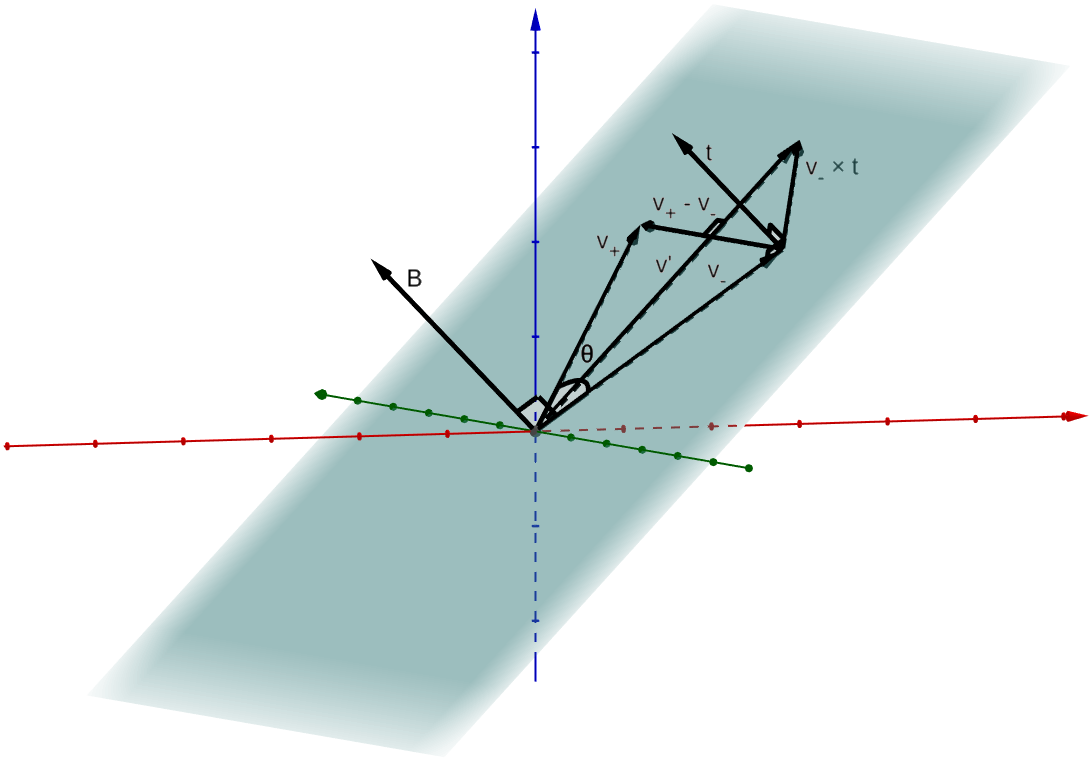
\includegraphics[width=\textwidth]{Boris-rotation-3D}
  \caption{Boris rotation construction in 3D}%
  \label{fig:Boris-rotation-3D}%
\end{figure}

As can be seen in \cref{fig:Boris-rotation-3D},
\(\vb{v}_+ - \vb{v}_- \parallel \vb{v}' \cp \vb{B}\). This encourages
the following notation: \(\vb{v}_+ - \vb{v}_- \equiv \vb{v}' \cp \vb{s}\),
where \(\vb{s}\) can be determined by the condition that
\(|\vb{v}_+|^2 = |\vb{v}_-|^2\). Thus, expanding \(\vb{v}' \cp \vb{s}\) gives
\[
\vb{v}' \cp \vb{s} = (\vb{v}_- + \vb{v}_- \cp \vb{t}) \cp \vb{s} =
\vb{v}_- \cp \vb{s} + \vb{t} \underbrace{(\vb{v}_- \vdot \vb{s})}_0 - \vb{v}_- (\vb{t} \vdot \vb{s})
\]

\begin{wrapfigure}[15]{r}{0.4\textwidth}
  \centering
  \subimport{../figures/}{Boris-rotation-construction}%
  \caption{The velocities projected in the plane perpendicular to \(\vb{B}\)}\label{fig:Boris-rotation-construction}%
\end{wrapfigure}

and if we consider the definition for \(\vb{s}\)
\[
\vb{v}_+ = \vb{v}_- + \vb{v}' \cp \vb{s} =
\vb{v}_- + \vb{v}_- \cp \vb{s} - \vb{v}_- (\vb{t} \vdot \vb{s})\,.
\]
Taking the scalar product with \(\vb{v}_-\) gives
\[
\vb{v}_+ \vdot \vb{v}_- = |\vb{v}_-|^2 - |\vb{v}_-|^2 (\vb{t} \vdot \vb{s})
\]
or
\[
|\vb{v}_-|^2 \cos{\theta} = |\vb{v}_-|^2 (1 - \vb{t} \vdot \vb{s})\,.
\]

Using the trigonometry identity
\[
\cos{\theta} = \frac{1-\tan^2{\frac{\theta}{2}}}{1+\tan^2{\frac{\theta}{2}}}\,,
\]
we obtain
\[
\vb{t} \vdot \vb{s} = 1 - \frac{1-\tan^2{\frac{\theta}{2}}}{1+\tan^2{\frac{\theta}{2}}}\,,
\]
which is equivalent to
\[
\vb{t} \vdot \vb{s} = \frac{2 t^2}{1+t^2}
\]
and thus we obtain that
\[
\vb{s} = \frac{2 \vb{t}}{1+t^2}\,.
\]

As a summary, the Boris push algorithm solves \cref{eq:lorentz-discrete-v} with the following steps:
\begin{enumerate}
  \item \(\vb{v}^- = \vb{v}_{n-1/2} + \frac{q \vb{E}}{m} \frac{\Delta t}{2}\)
  \item rotate \(\vb{v}^-\) to obtain \(\vb{v}^+\) using
  \begin{enumerate}
    \item \(\vb{v}' = \vb{v}^- + \vb{v}^- \cp \vb{t}\), where \(\vb{t} = \frac{q \vb{B}}{m} \frac{\Delta t}{2}\)
    \item \(\vb{v}^+ = \vb{v}^- + \vb{v}' \cp \vb{s}\), where \(\vb{s} = \frac{2 \vb{t}}{1+t^2}\)
  \end{enumerate}
  \item \(\vb{v}_{n+1/2} = \vb{v}^+ + \frac{q \vb{E}}{m} \frac{\Delta t}{2}\)
\end{enumerate}

\subsection{Conservation properties}

When solving (continuous) differential equations with (discrete) numerical methods,
an important aspect is that we want the algorithm to be as close as possible to
the original continuous system in terms of symmetries and conserved quantities.

In what follows we will look at the conservation properties of the Boris push
and show why are they important for simulating the dynamics of charged particles
following the ideas presented in~\textcite{qin_whyboris_2013}.

Mathematically speaking, a Hamiltonian system is given by the phase space (an
even dimensional manifold\footnote{A manifold is a topological space that is locally Euclidean}),
a symplectic structure on it and the Hamiltonian
function~\autocite[160]{arnold_mathematicalmethods_1989}.
In order to explain what the symplectic structure is, we will start with a short
discussion about 2-forms~\autocite[164]{arnold_mathematicalmethods_1989}.

\begin{definition*}
  An exterior form of degree 2 (or a 2-form) is a function of pairs of vectors
  \(\omega^2: \mathbb{R}^n \cp \mathbb{R}^n\), which is bilinear and skew symmetric:
  \begin{align*}
  \omega^2(\lambda_1 \vb*{\xi}_1 + \lambda_2 \vb*{\xi}_2, \vb*{\xi}_3) &=
  \lambda_1 \omega^2(\vb*{\xi}_1, \vb*{\xi}_3) + \lambda_2 \omega^2(\vb*{\xi}_2, \vb*{\xi}_3) \\
  \omega^2(\vb*{\xi}_1,\vb*{\xi}_2) &= -\omega^2(\vb*{\xi}_2, \vb*{\xi}_1)\,,
  \end{align*}
  \(\forall \lambda_{1,2} \in \mathbb{R}, \vb*{\xi}_{1,2,3} \in \mathbb{R}^n\).
\end{definition*}

As an example of a 2-form in \(n=2\) dimensions is given by the \emph{oriented area} spanned by 2 vectors
in the (oriented) euclidean plane \(\mathbb{R}^2\).
Let us consider
\[
\vb*{\xi} = \mqty(\xi_1 \\ \xi_2), \qquad
\vb*{\eta} = \mqty(\eta_1 \\ \eta_2)\,,
\]
then the oriented are determined by the two vectors is given by
the determinant~\autocite{golomb_proofwords_1985}
\[
S(\vb*{\xi},\vb*{\eta}) = \det\mqty(\xi_1 & \eta_1 \\ \xi_2 & \eta_2)
= \xi_1 \eta_2 - \xi_2 \eta_1\,.
\]

If we now consider an \(n\)-dimensional phase space with the coordinates \(p_i,q_i\) as in~\textcite[183]{hairer_geometricnumerical_2006},
we will have the projections of the hyper-parallelogram on the coordinate planes
\[
\omega(\vb*{\xi},\vb*{\eta}) = \sum_{i=1}^n \det\mqty(\xi_i^p & \eta_i^q \\ \xi_i^q & \eta_i^p) =
\sum_{i=1}^n \left(\xi_i^p \eta_i^q - \xi_i^q \eta_i^p\right)\,.
\]

This bilinear form can also be written is matrix notation as
\[
\omega(\vb*{\xi},\vb*{\eta}) = \vb*{\xi}^T J \vb*{\eta}\,,
\quad \text{where} \quad J = \mqty(0 & I \\ -I & 0)\,,
\]
with \(I\) the identity matrix in \(n\) dimensions.

\begin{definition}
  A linear map \(A: \mathbb{R}^{2d} \to \mathbb{R}^{2d}\) is called
  \emph{symplectic} if
  \[
    A^T J A = J\,,
  \]
  or \(\omega(A\vb*{\xi}, A\vb*{\eta}) = \omega(\vb*{\xi},\vb*{\eta})\,,\
  \forall \vb*{\xi}, \vb*{\eta} \in \mathbb{R}^{2d}\).
\end{definition}

An useful example that illustrates the concept is given in the case of \(d=1\),
where symplecticity implies area conservation under the given
linear transformation. Expanding on the above examples,
for the \(d>1\) case, it would imply the conservation of the sum
of the respective projected areas.

As we have seen from the beggining of this chapter, differentiable
functions are often approximated using linear maps. This provides
the motivation for extending the above definition to the non-linear case.

\begin{definition}
  A differentiable map \(g:U \to \mathbb{R}^{2d}\), with \(U \subset \mathbb{R}^{2d}\) an open set, is called \emph{symplectic}
  if its corresponding Jacobian matrix \(g'(\vb{p},\vb{q})\) is evereywhere symplectic, i.e.
  \[
    {g'(\vb{p},\vb{q})}^T J g'(\vb{p},\vb{q}) = J
  \]
  or \(\omega(g'(\vb{p},\vb{q})\vb*{\xi}, g'(\vb{p},\vb{q})\vb*{\eta}) =
  \omega(\vb*{\xi},\vb*{\eta})\).
\end{definition}

Having defined symplecticity, we will now try to check if the Boris
push algorithm is symplectic. For this task we begin with rewriting
\cref{eq:lorentz-discrete-v} in a more convenient form
\[
\vb{v}_{n+1/2} - \frac{q \Delta t}{2m} \vb{v}_{n+1/2} \cp \vb{B} =
\vb{v}_{n-1/2} - \frac{q \Delta t}{2m} \vb{v}_{n-1/2} \cp \vb{B}
+ \frac{q \Delta t}{m} \vb{E}\,.
\]

In order to manipulate the above more easily, it is useful to introduce the following definition~\autocite[289]{marsden_introductionmechanics_1999}

\begin{definition}
  The \emph{hat map} \(\hat{}: \mathbb{R}^3 \to \mathfrak{so}(3)\) is a
  vector space isomorphism that identifies the Lie algebra \(\mathfrak{so}(3)\)
  of \(SO(3)\) with \(\mathbb{R}^3\). If we consider
  \(\vb{v} = (v_1,v_2,v_3) \in \mathbb{R}^3\), then the hat map
  is given by
  \[
    \hat{\vb{v}} =
    \begin{pmatrix}
      \phantom{-}0\phantom{_1} & -v_3           & \phantom{-}v_2 \\
      \phantom{-}v_3 & \phantom{-}0\phantom{_1} &           -v_1 \\
            -v_2     & \phantom{-}v_1 &\phantom{-}0\phantom{_1}
    \end{pmatrix}\,.
  \]
\end{definition}

We can observe that
\[
\hat{\vb{v}} \vb{w} = \vb{v} \cp \vb{w}
\]
characterizes the isomorphism. Comparing
\[
\hat{\vb{v}} \vb{w} =
\begin{pmatrix}
  \phantom{-}0\phantom{_1} & -v_3           & \phantom{-}v_2 \\
  \phantom{-}v_3 & \phantom{-}0\phantom{_1} &           -v_1 \\
        -v_2     & \phantom{-}v_1 &\phantom{-}0\phantom{_1}
\end{pmatrix}
\begin{pmatrix}
  w_1 \\
  w_2 \\
  w_3
\end{pmatrix}
=
\begin{pmatrix}
            -v_3 w_2 + v_2 w_3 \\
  \phantom{-}v_3 w_1 - v_1 w_3 \\
            -v_2 w_1 + v_1 w_2
\end{pmatrix}
\]
with
\[
(\vb{v} \cp \vb{w}) = \vb{e}_i \epsilon_{ijk} v_j w_k =
\vb{e}_1 (v_2 w_3 - v_3 w_2) + \vb{e}_2 (v_3 w_1 - v_1 w_3) +
\vb{e}_3 (v_1 w_2 - v_2 w_1)
\]
we can see that this is indeed true.

Thus, if we consider \(\mathbb{R}^3\) together with the cross product,
the hat map \(\hat{}\)\ becomes a Lie algebra isomorphism and we
can identify \(\mathfrak{so}(3)\) with \(\mathbb{R}^3\) having the
cross product as Lie bracket.

\section{The field solver}

\section{A survey of available PIC codes}

Frequently used simulation programs include

\begin{table}
  \begin{tabular}{l l l l}
  \toprule
  \textbf{Name} & \textbf{Type} & \textbf{GPU ready} & \textbf{Scalability}\\
  \midrule
  EPOCH & EM 3D & No & MPI\\
  Osiris & EM 3D, RZ*, RZ** & No & MPI, OpenMP, SIMD\\
  VSim & EM 3D & No & MPI\\
  PIConGPU & EM 3D & Yes & MPI, CUDA-ALPAKA\\
  FBPIC & EM 3D, RZ*** & Yes & MPI, NUMBA\\
  Warp & EM 3D, PS*, RZ*, RZ** & No & MPI, OpenMP\\
  WarpX & EM 3D, PS*, RZ*, RZ** & No & MPI, OpenMP, SIMD\\
  VPIC & EM 3D & No & MPI, pthreads, SIMD\\
  Architect & EM RZ & No & MPI\\
  Wake & QS RZ & No & MPI\\
  QuickPIc & QS RZ & No & MPI\\
  PICLS & EM 3D & No & MPI\\
  \bottomrule
  \end{tabular}
  \caption{Commonly used simulation programs}%
  \label{tab:pic-software}
\end{table}

In the above table we used the following abbreviations
\begin{itemize}
    \item EM: Electromagnetic PIC
    \item QS: Quasi-Static PIC
    \item 3D: Cartesian coordinates, up to 3D
    \item RZ: Cylindrical geometry with FDTD method in \(r\) and \(z\) directions
    \item RZ*: Cylindrical geometry with Fourier azimuthal decomposition
    \item RZ**: Cylindrical geometry with FDTD method in \(r\) direction
                and FFT-based pseudo-spectral method in \(z\) direction
    \item RZ***: Cylindrical geometry with Henkel transform in \(r\) direction
                and FFT-based pseudo-spectral method in \(z\) direction
    \item PS: Pseudo-spectral Maxwell solver with golbal Fourier transform
    \item PS*: Pseudo-spectral Maxwell solver with domain decomposition and local Fourier transform
\end{itemize}

% tabel ✓
% grafic scalabilitate osiris
% mentiune osiris/grup lisabona in ELI whitebook
% coduri de tip WARP de la Bella, citare JL Vay & H Vincenti, picsar ref Vincenti
% referinta tdr eli-np negoita

\section{EPOCH}

\end{document}
